%Introduction

The human brain can be analyzed from different points of views. Some disciplines look at it from the outside, and try to understand how it responds to stimuli, how it behaves on different conditions, how it adapts to new contexts and how it changes over time. Some disciplines look at it at cellular and molecular level, trying to understand the chemical reactions that go on inside each cell making it work. Others analyze the activity of a groups of cells analyzing how they cooperate. Some focus on larger structures composed of several cells, trying to understand how they connect to each other and how the different types of organs complement each other. It is of special interest seeing how it matures over time, and how it recovers from traumatic events. Additionally it is important to analyze how it degenerates over time, and what diseases can affect it in order to create treatments and help the brain heal. 
These tasks are carried out by different specialists in very different environments. There are also a wide range of tools designed for studying the brain, from microscopes and voltage clamping techniques, to psychology instruments. There are also studies based on animals with similar structures or even electronics circuits specifically built to emulate the human brain. 

This shows that understanding the brain is far from easy, and that it involves an enormous amount of skills, tools and knowledge. It can also be seen that all of these information gathered from different perspectives must be integrated in other to get a full understanding. This will require teams from diverse specialties and contexts to work together, each providing one piece of the puzzle. 

This task will also require support from computational tools in order to be efficient. These tools should allow experts from different contexts to be productive as teams and to integrate data acquired using a wide array of methods. Data itself will be highly heterogeneous and there will be lots of it. As tools advance we become more efficient at making experiments and generating data, and the bottleneck has become analyzing it. In other words, data is acquired at a fastest rate than it can be understood. 

This is indeed a complex scenario, and it is evident that a single software tool will not be able to solve all the problems. Tackling the whole problem at once is also an impossible tasks. We need to break down the problem into simpler tasks that can be attacked without loosing the big picture. Doing this analysis is itself a challenging task, that can't be addressed lightly. Fortunately this kind of problems are found in several business applications and  software engineering techniques that can manage them have been developed. 

As mentioned previously, the problem of integrating brain data involves several points of view and several types of work-flows. This is a clear signal of the need for different applications instead of a single, all-mighty application. Nevertheless these applications will likely share several aspects. Analyzing these commonalities and differences is the first step towards a solution to the problem. 
Methodologies to do this can be borrowed from software product line engineering \autocite{pohl_software_2005}, model driven software engineering \autocite{brambilla_model-driven_2012} and generative programming \autocite{czarnecki_generative_2000}. 

The first task will be the scoping of the domain and the selection of a domain where a it is feasible to make a contribution. Afterwards the commonalities and differences in the needs of the different stake-holders, work-flows, and data in the selected domain are analyzed in order to create a feature model. This model will be the basis for a proposal of an applications family, where each application addresses a particular problem inside the domain. 


\section{Domain Engineering}

Domain Engineering is the practice of selecting and characterizing the domain in which the application family will be built. A good description of the steps required for this task can be found in \autocite{czarnecki_generative_2000}. We will follow these steps in order to identify the domain where we will work on the rest of the thesis.

\subsection{Domain Scoping}

As noted previously brain research involves several specialties, skills and techniques. It could be argued that because the brain is involved in almost every human action, all human and social sciences are at the end studying the brain. However in this project we will focus on more direct studies of the human brain. In particular we want to analyze its physical structure. Under this condition there are still a broad ways of looking at it.

In domain engineering the decision of where to focus must be also influenced by the strengths and experience of the organization, in this case our research group. Previous projects of the group (\footnote{Proyectos de Darwin, Jaime, Marcela}) have principally focused on analysis of medical images at m.m. scale, acquired by CT and MRI machines. We have good relationships with radiology departments at several hospitals and therefore access to images and, more critical, domain experts. MRI is an specially interesting technique as it does not produce ionizing radiation, and therefore is harmless for the subject. While CT and general x-rays involve radiating the human body. This is not harmful at small doses but the effects may accumulate over time. Therefore these techniques must be used with care and only when there is a valid medical reason that justifies it. On the other side, MRI scans can be applied to any subject and there is no need for a medical justification (but probably the study must be approved by an ethical committee). MRI scanners are also versatile machines which can acquire numerous kinds of images. Structural images can be acquired at different configurations which provides better contrast for different tissues or molecules. Advanced techniques grant the ability to do spectroscopy in order to characterize the composition of specific areas of the brain. By using contrast agents it is also possible to precisely locate specific proteins, cells or structures. 
For these reasons we chose to focus our development on images acquired by MRI. We also chose to focus on T1 and T2 weighted structural images, Diffusion weighted images and BOLD f-MRI. This decision was also caused by the previous experiences in the group, but nevertheless keep in mind that domain definition and scoping is an iterative process, and therefore this decision will certainly be revisited in the future.

An objective of the project from the start has been the integration of data, therefore even though we are focusing on MRI data, we need additional data to provide context and therefore a more complete picture. Recall that one of our hypotheses is that the brain is better understood by teams of specialists who can bring different perspectives. One of our challenges was linking structure and function of the brain. This function of the brain may signify quick reactions to stimuli, like for example catching a ball, all the way to complex social behaviors over several years. This kind of data can be collected by economists, psychologists, epidemiologists, and sociologists among others. This information can be very complex, but a non trivial subset of it consists of numerical, nominal and ordinal variables which can be registered in spreadsheet tables. We will attempt to integrate data from these diverse set of disciplines if it is presented in a table-like format, but we will not try to interpret the data in any way. This responsibility will fall on end users. 

Finally there is another important kind of data we want to consider as it provides a perfect link between structure and functioning of the brain. This is, data from TMS exams. We are very lucky to have access to neurophysiologists specialized in this kind of exams, which can further enlighten the functioning of the brain and its relationship to its structure. To recapitulate, the current project is going to consider the following kinds of data:

\begin{itemize}
\item MRI brain images
\begin{itemize}
\item Structural T1 and T2 weighted
\item Diffusion Weighted Images
\item Functional MRI
\end{itemize}
\item TMS exams
\item Tabular data from other disciplines
\begin{itemize}
\item Nominal variables
\item Ordinal variables
\item Numeric variables
\end{itemize}
\end{itemize}  

Another key aspect of domain scoping is identifying stakeholders and their interests. As mentioned earlier the brain can be studied from a clinical perspective with the aim of healing it. This is usually done case by case in hospitals or health centers. While this is a very important activity, we are most interested in analyzing cohorts of subjects. Also, getting into the clinical diagnosis practice would involve dealing with significant more regulations, which would increase the complexity of the project. The other major group of users of medical images are brain researchers. As was described in the introduction chapter, this is our main target. In particular we focus on interdisciplinary brain research projects, where there is data from multiple subjects and different nature, and an interest to find relationships across the different dimensions. The data available for each subject should be reasonably consistent across the complete sample. The stakeholders are therefore the researchers involved in such a project. These researchers can come from several backgrounds, which include

\begin{itemize}
\item Radiologists
\item Physicians
\item Psychologists
\item Physiologists
\item Epidemiologists
\item Economists
\end{itemize}

Their goals are extracting information and meaning out of the data. As mentioned earlier this is the core problem that lead to the birth of visual analytics. However it is crucial to understand that each specialist will inevitably have his own interests and his own methods. The real challenge is creating a common framework that would help and encourage specialists from different disciplines to work together and collaborate efficiently. Therefore in order to achieve the ultimate goal it is necessary to improve communication inside the team, and to encourage specialists to go out of their zone of comfort and ask questions about data they don't usually look at. However this must be done responsibly, the objective is not to ignore the true specialists in a particular kind of data, but the opposite, improve communication between these specialists. 

Each specialty also incorporates their own work-flows. These include protocols for data acquisition, pre-processing, storage, processing and analysis. As mentioned in the introduction analysis usually take the form of null hypothesis significance testing, and plenty of tools exist for this purpose. Nonetheless exploratory data analysis is also very important, specially when huge amounts of data are available. Traditionally data acquisition was also tuned for the testing of particular hypotheses, but it is becoming common to acquire data in a more open-ended fashion. In this project we will not deal with data acquisition nor data processing. The focus is on visual exploratory analysis of already processed data.  

In conclusion, the scope of the project is now bounded in data types (MRI and tabular), stakeholders (interdisciplinary research groups), and tasks (visual exploratory analysis). However, it is worth reiterating that domain scoping is an iterative process, which has to go on for the duration of the project. 

Domain Model

%- Stakeholders
%- Users
%-- points of view
%-- activities
%-- teams
%-- selfish
%
%-- Alternatives
%-- choose
%- Scope
%-- Alternatives
%-- Choose


\subsection{Domain Modeling}

After choosing and bounding the domain we need to go deeper into its characterization. This task is accomplished by reading bibliography in the domain, contacting stakeholders and analyzing existing software. The details of the information gathered at this stage can be found in chapter \ref{chap_related}. In this section we will describe the domain based on that information.

%Workflow
A typical MRI experiment starts with a set of hypotheses which want to be tested on a target population. A protocol is designed to test the hypotheses and if possible correct sample sizes are calculated. Afterwards participants are recruited, and data is collected. This process is not always smooth, and often corrections must be made and acquisition repeated. Inevitable some data will not be useful and some participants will have to be removed from the study. Data acquired from the MRI machine must be taken out, stored and processed. There are different processing pipelines for different kinds of images, but most of them are designed to perform statistical tests using the images and some external variables. The results of the statistical tests have to be interpreted in order to write the report of the experiment and what we learned from it.

As mentioned in chapter \ref{chap_intro} we intend to use data collected in these experiments as well as data collected in open-ended fashion to perform exploratory and data-driven analyzes. Still, most of the steps in traditional experiments will be the same, and we are required to play nice with existing tools and work-flows. 

\begin{figure}
\centering
\begin{subfigure}[b]{0.9\textwidth}
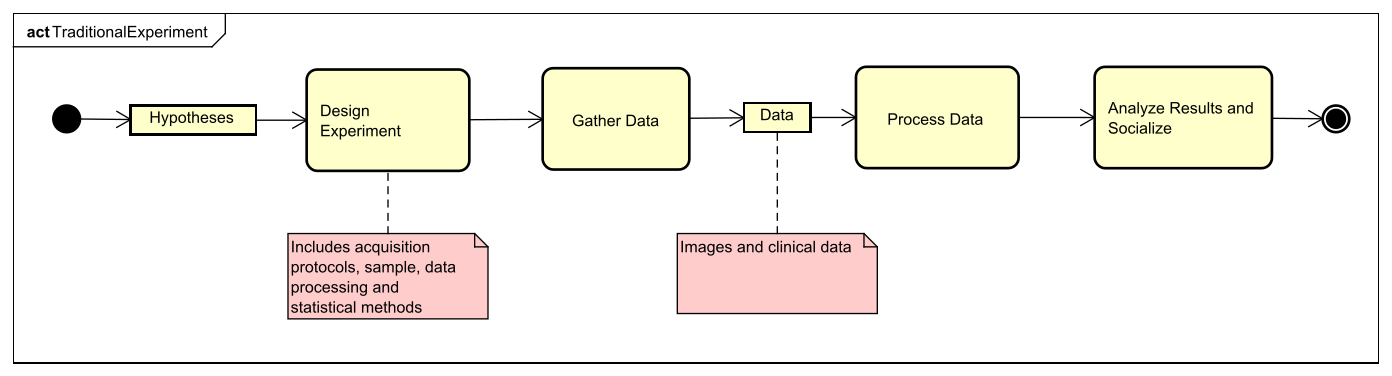
\includegraphics[width=\textwidth]{domain/TraditionalExperiment}
\caption{The Scientific Method workflow}	
\end{subfigure}

\begin{subfigure}[b]{0.9\textwidth}
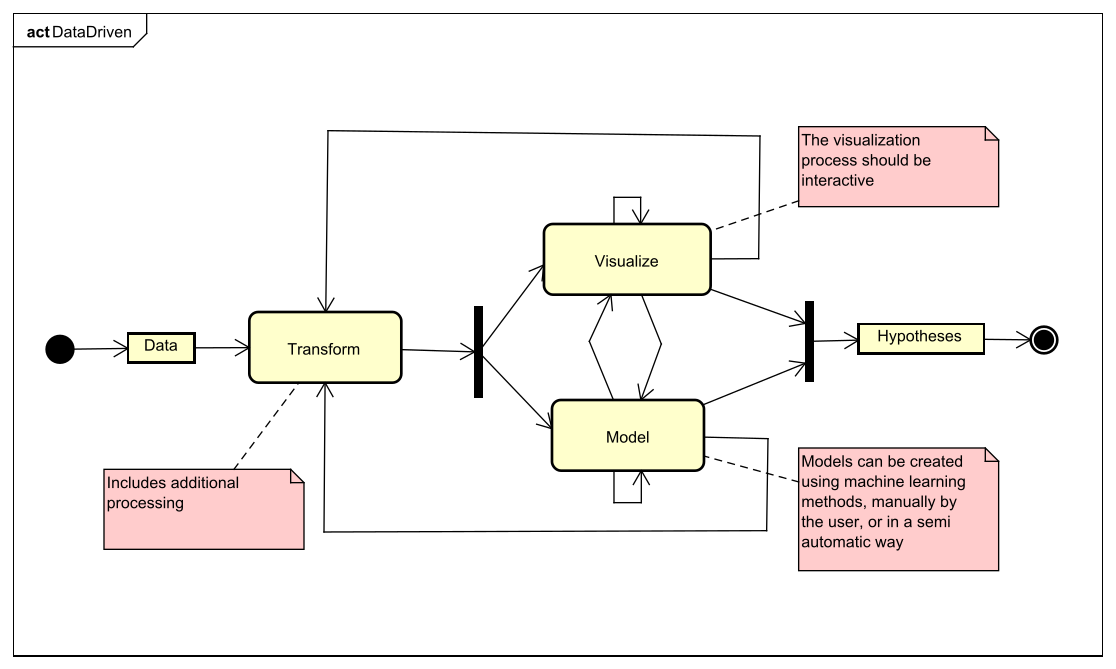
\includegraphics[width=\textwidth]{domain/DataDriven}	
\caption{The Data Driven workflow}	
\end{subfigure}

\caption{\label{fig_workflows}Comparison between scientific method and data driven research. It can be seen that the scientific method is linear, and uses the data exactly once, while in data driven research the process is highly iterative and data is used multiple times.}
\end{figure}

Figure \ref{fig_workflows} shows the comparison of the two work-flows. It can be seen that the input for traditional experiments are hypotheses, while the output of data driven research are also hypotheses. Meanwhile the input to the data-driven research loop is data, which as mentioned earlier can come from finished experiments. This shows how both work-flows can complement each other. Also notice data processing takes place at both loops. The meaning is that the data-driven and hypotheses-driven research domains are deeply linked.  

%Data
\begin{figure}
\centering
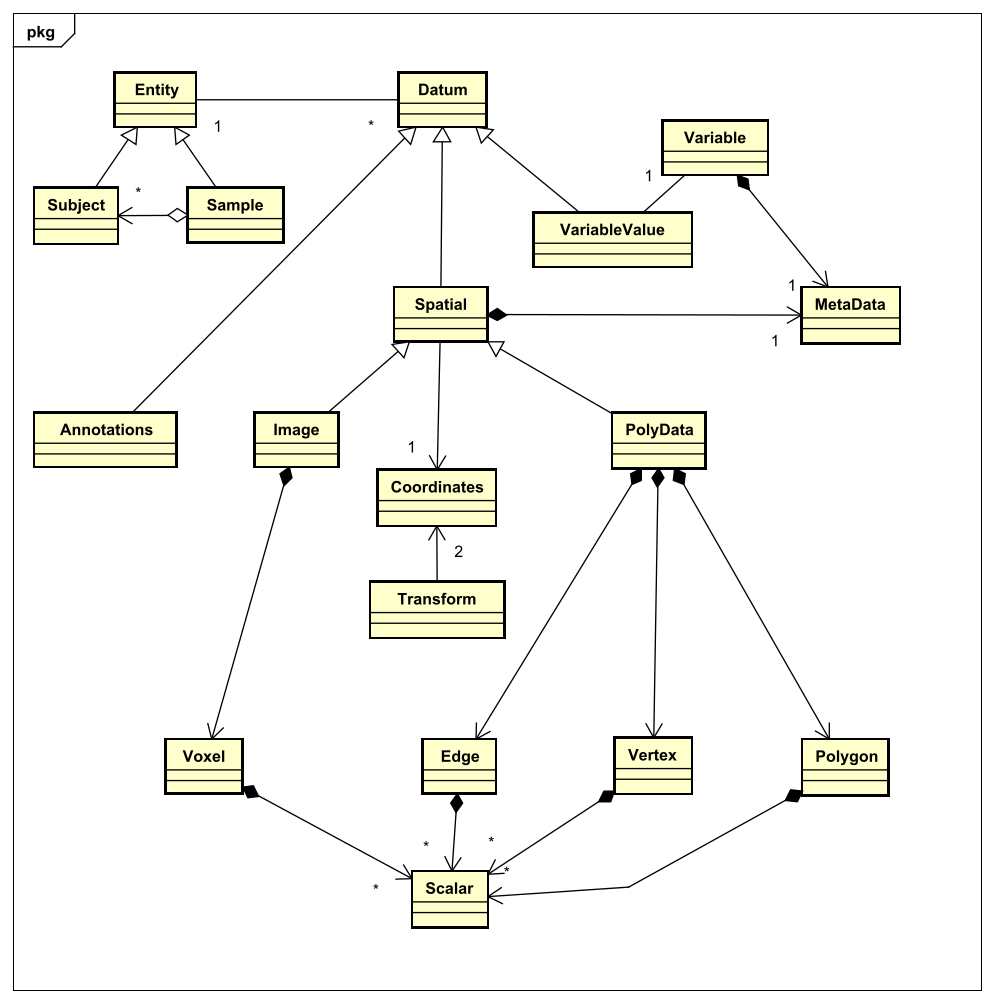
\includegraphics[width=0.9\textwidth]{domain/ClassDiagramData}
\caption{\label{fig_datum_class} Domain data model. Each individual datum is associated to either a sample or a subject. A datum can be the value of variables, or a spatial structure. Variables can be nominal, ordinal or real, while spatial structures may be images or polydata. Spatial structures must always be associated to a coordinate system in which they are defined. Transforms may be used to move spatial objects from one coordinate system to another.}
\end{figure}

Data is the most important object in our domain, so we need to characterize it in a more precise way. Inside our scope, data is a collection of data-points each of whom is also called a datum. Figure \ref{fig_datum_class} shows a class diagram of a datum. The highlights of the drawing are

%definitions

\begin{itemize}
\item Each datum is associated to an Entity
\item An entity may be a single subject or a sample
\item A sample is composed of several subjects, each subject can belong to several samples
\item The two main kind of datum (in our scope) are spatial and variable values
\item An spatial datum may be an image or polydata
\item All spatial objects are associated with a coordinates system
\item Transforms can be used to map between two coordinate systems
\item Images are composed of voxels
\item Polydata are collections of vertices, edges and polygons
\item Voxels, edges, vertices and polygons may be associated with one or more scalar values.
\item All spatial data must me associated to some meta-data
\item VariableValues belong to a certain variable
\item Each variable is associated with meta-data  
\item Data which is neither a VariableValue nor a spatial object can be encoded into textual annotations
\end{itemize} 

Meta-data plays an important role. On the spatial side it lets us identify which images or polydata can be analyzed together. In other words, it is through this metadata that it becomes to possible to identify matching pieces of information belonging to different subjects. In the case of variables, the metadata provides important information on how to interpret the values that the variable takes. Some concrete examples of data are
\begin{itemize}
\item Image:
\begin{itemize}
\item T1-weighted structural image
\item Color coded DTI image with 3 scalar values per voxel
\item A label map where each voxel contains a value indicating to what structure it belongs 
\end{itemize}
\item PolyData:
\begin{itemize}
\item A group of fibers from a tratography
\item Cerebral cortex surface reconstruction
\item An iso-surface representing an activated area in a fMRI paradigm
\end{itemize}
\item Variable:
\begin{itemize}
\item Gender
\item Height
\item Score at a neuropsychological test
\item Time it took to complete a marathon
\item Level of pain in a likert scale
\item Place of birth
\item Latency in a TMS test
\end{itemize}
\end{itemize}

%Processing

It can be seen that this simple structure allows us to represent a wide array of data types. Some of this data are raw values that can be found directly, and some are the results of processing steps applied to raw data. As mentioned earlier we don't expect our system to do data processing, but there is a close relationship with these kind of procedures. In fact the system should be able to do additional processing when it is required, but delegating this task to third party tools fit for the job. As seen in figure \ref{fig_workflows} processed data is fed back into the system, and afterwards can be used in the same way as raw data. Some examples of the processing steps that we expect to utilize are

\begin{itemize}
\item Estimating diffusion models (like DTI)
\item Reconstructing tractographies
\item Segmentation of structural images
\item Reconstruction of segmented structures
\item Cortical surface reconstruction and parcellation, as done in FreeSurfer
\item Linear and non linear registration
\item Applying transforms to move spatial objects to a different coordinate system
\item Creating frequency maps from several co-registered label maps.
\item Filtering tractographies
\item Calculating volumes, areas, and mean values of a scalar, for a given surface.
\item Statistical tests involving images from two different groups (like VBM, or second level fMRI analysis)
\item Clustering on a set of variables
\item Fitting of statistical models on a set of variables
\end{itemize}

As usual, this is not an exhaustive nor final list. As the project evolves it is likely that we will have to incorporate additional processing algorithms. The vision is to take advantage of available tools whenever possible. Fortunately there is an ample set of high quality open source tools available as was shown on chapter \ref{chap_related}.

%Stake Holders

The expected users in this project are research groups containing specialists from different backgrounds, however there are several other stakeholders who must be considered in the development of the project. The data comes from real participants, which may have concerns about too many people looking at their data. On the other side the project managers and funding agencies want the best return of investment possible, which means extracting as much information and knowledge as possible from the collected data. Usually the participants of the experiment, whose data was collected, signed a consent which permits some use of the data. The contents and permissions granted by these agreements have to be taken into account. A common trade-off is for the participants to grant unlimited usage of the data as long as it is anonymized. In theory it shouldn't be possible to figure out the true identity of a subject based on anonymized data, but this is hard to guarantee in practice, specially when so much complementary data can be obtained from third parties \autocite{singel_netflix_2009}. Also the anonymization procedure involves adding noise to the data, which will have an impact on the analysis. When data is analyzed as extensively and deeply as we are proposing, the risk of deanonimyzing the subjects increases. Therefore measures have to be taken into account to increase protection, either by limiting access to the data to a small group of researchers, or increasing the strength of anonymization measures. 

Another possible concern is the loss of statistical rigor. As shown in figure \ref{fig_workflows} traditional research is based on the fact that data is used once for a statistical test. In this case meaningful metrics of significance can be reported. However when data is used more than once we fall into a multiple comparisons problem \footnote{quote}, where the chances of false positives increase and therefore corrections should be applied to significance metrics. Nevertheless the scientific community is concerned that researchers will not apply corrections and report results which are not really accurate. While we can't do anything against dishonest researchers, the proposed platforms may make it easier to cheat in order to get more impressive results. As mentioned on the introduction, this problem arises from publication bias. Under this situation some researchers may believe that the best way to guarantee a publication is by reporting some fantastic significance metrics, and try everything they can to get this values. It is key here to remember that the proposed platform is meant to be used as a mean for generating hypotheses, not to formally proof them. While the analysis carried on in the platform may provide evidence in favor of some hypothesis, it is also highly susceptible to the multiple comparisons problems. Therefore it is necessary to be skeptical about the data, and always validate hypotheses using external datasets.  

Understanding the main users of the application is at the core of the design process. Recall that we are using a user centered design methodology, involving end-users constantly during the design process. Understanding the users is also central for the domain-modeling activity. This includes examining their current workflows and tools is the starting point for this. We accomplished this by visiting several labs and hospitals, and watching several experiments, from data acquisition to data analysis. The knowledge from other works in visual analytics can also be applied here. 

First of all, brain researchers are human. As humans we all have limitations on the amount of information we can keep in memory and our ability to concentrate. The analysis platform should help mitigate this by unloading the memory of the specialist to the screen. All of the required information should be visible or easy to access. In order to avoid distractions, it is important to have a fast response time. If the application constantly makes the user wait, then probably he will loose interest and move to another task. A peculiarity of brain researchers is that they are very busy, and usually there is no time in their agenda reserved for data exploration. This activity is carried on at the spaces between tasks, and even tough there is a high chance of being interrupted by students or colleagues. Therefore it is essential for the platform to support work at different intervals and under constant interruptions. In practice this means efficient facilities to save and restore work, as well as additional information to recover the flow from the last session. 

Visual Analytics recognizes that humans have limited cognitive capacity, and the point is to make the best possible use of it. One key point here is that the cognitive budget should be spent on the data and not on the tools. This means that the experts should always be thinking about the underlying data, not on details of the tool used to look at it. Consider for example watching TV, how much time do you spend thinking on details of the tv-set? If tools require complex commands, or the controls are not intuitive, the attention will have to shift to how to accomplish a task in the tool. Another key concept required here is that tools should adapt to users, instead of making users adapt to tools \autocite{norman_design_2002}. This also means that technical details or repetitive actions should be solved automatically. For example there are dozens of image data formats available, and each tool works with some of them. This forces the user to spend time thinking which tool is appropriate for each format, or if there is a need to convert it. The same goes to dealing with files in file system, users should not be thinking on what is the best way to organize files so that they can be easily found afterwards. 

On the other side, researchers are the most fit, if not the only, who can interpret and make sense of this vast amount of data. As the data grows larger, chances of patterns appearing by chance also increase. Only experts can discriminate between true interesting findings and random noise. They can do this because they possess a strong theoretical background, which can be used to give meaning to data. They also have experience working with patients and data, and therefore can associate data from a study to past experiences and close cases. From all these they have also developed an intuition, that can guide them to interesting places. Given the familiarity with the data, experts can quickly spot common mistakes or find simple explanations to what may appear surprising for an outsider. 

In summary some of the main characteristics of a hypothetical user are

\begin{itemize}
\item Limited memory
\item Limited concentration
\item Busy schedule
\item Not interested in technical details
\item Background knowledge
\item Experience
\item Intuition
\end{itemize}

%Group memebrs also belong to other groups

%Florero, evidencia de los argumentos, no recurrir a la memoria, sino tener la informacion visible

% groups

Groups of experts are also interesting because their expertise are on different areas. Therefore while they are deeply familiarized with some aspects of the data, other aspects are foreign. In a similar way each expert is inclined to analyze data of a particular nature or in a particular way. Some teams are composed of experts located far from each other. Often they don't even share the same mother language. Communication between the different members of the group is therefore challenging, as is reconciling their interests and objectives, and moving forward as a group. Communication is different when a link to the physical reality can be stablished \autocite{rojas_arredondo_dinamica_2010}. By having data easily available at a meeting, researchers can provide evidence to support their ideas, and in this way have a conversation rooted to reality, instead of relying on memory or notes. Also ideas or questions that come up during the conversation could be explored right away, which can lead to a more fluent and efficient work session. Visual Analytics recognizes the human visual system as the most effective channel to get information into the expert's mind. By using this channel efficiently we believe communication can be improved. Also by providing easy access experts, we may lower the resistance from experts to explore data from other fields by themselves, to follow-up with colleagues and bring them questions. Yet again, there exists the danger of some members of the group wanting to control their data, and don't liking the idea of non-experts looking at it because probably they will not understand it. We will have to wait and see how these kind of tools and environment affect group dynamics.


\bigskip

% Existing viualization applications
In chapter \ref{chap_intro} a review of the tools currently used in the domain was presented. These tools have several things in common and several differences as shown in figure X. While most of the processing tools provide utilities for batch processing several subjects, visualization are mostly available for a single subject or for the results of statistical tests. Going through visualizations of several subjects requires several steps and most of the time repeating work. Also while most of them permit the use of linear transform to move the data to a different coordinate system, the end user must specify the adequate transform for each case. These tools offer very good performance for quality control or publication graphs, but for exploratory analysis we require a more streamlined workflow, with minimal need for repetition, and limiting as much as possible the exposure of technical details to the user. In the world of statistical visualization there has been a bigger growth in interactive solutions. For example tableau can be used to create highly interactive dashboards for the exploration of large datasets. These dashboards display several coordinated views of the data and permit the user to interactively change parameters and therefore get visualizations tailored for the current question. We are interested in using these kind of techniques but extend them to be better integrated with spatial data. 

\begin{figure}
\centering
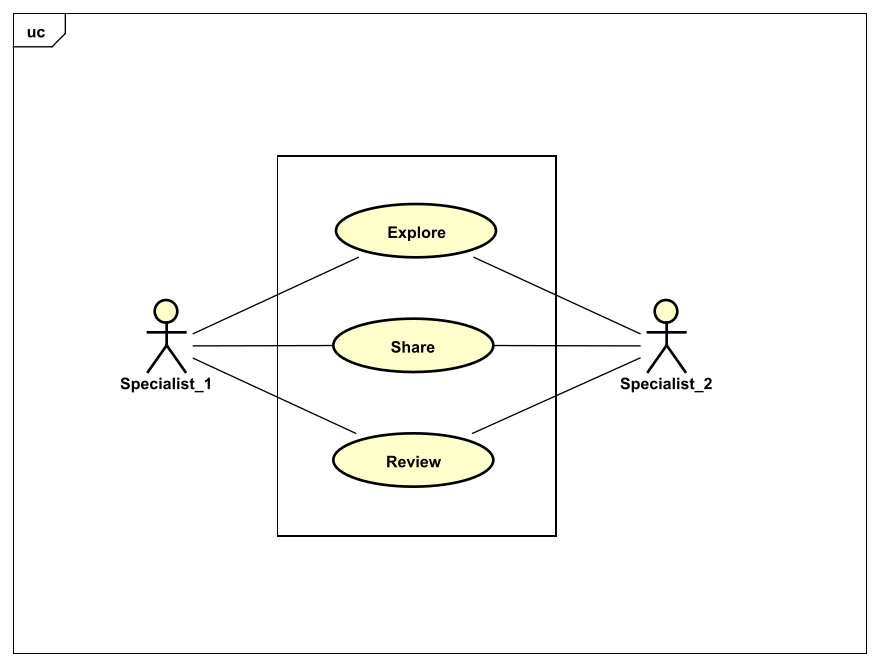
\includegraphics[width=0.5\textwidth]{domain/UseCaseGeneral}
\caption{The high level use cases of the system. It should allow each specialist to explore, share and review. Notice one expert may review the results from another member of the team.\label{fig_use_case_general}}
\end{figure}

\begin{figure}
\centering
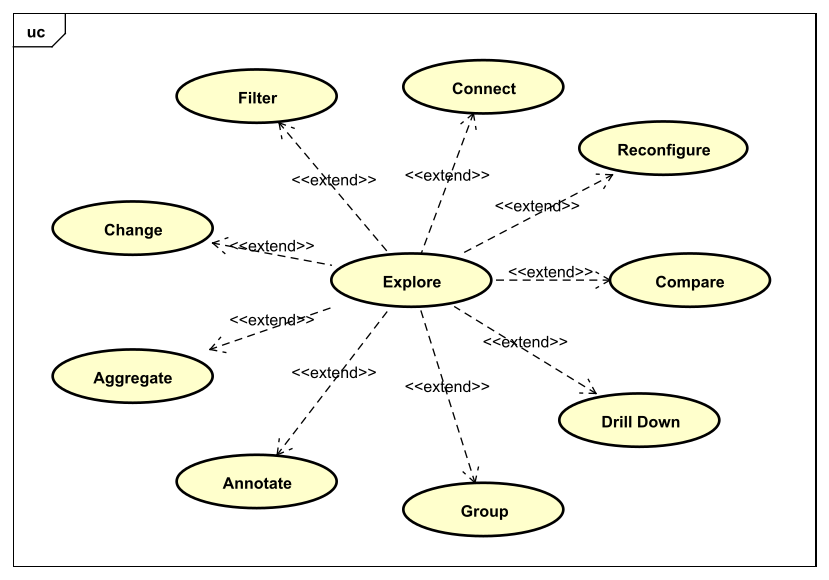
\includegraphics[width=0.9\textwidth]{domain/UseCaseExplore}
\caption{The explore activity can be achieved trough a combination of several analysis tasks. Connect: show similar data, Reconfigure: change arrangement of data, Compare: view differences and similarities between two entities, Drill Down: Get additional details, Group: join similar entities, Annotate: attach additional information to an entity, Aggregate: show less detail, Change: show something different, Filter: show something conditionally. Most of these tasks are taken from \autocite{yi_toward_2007}\label{fig_use_case_explore}}
\end{figure}

\begin{figure}
\centering
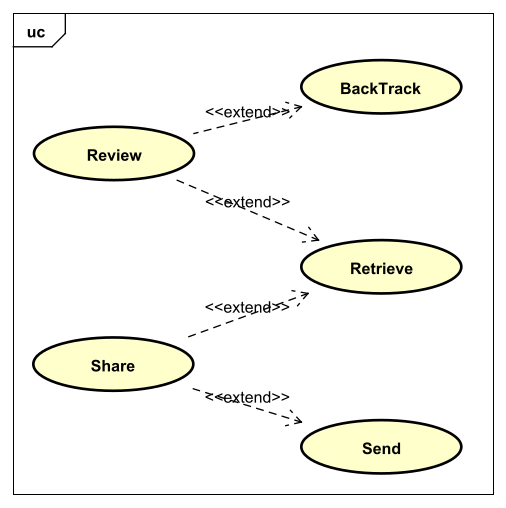
\includegraphics[width=0.5\textwidth]{domain/UseCaseShare}
\caption{The review and share use cases contain the following activities. BackTrack: reconstruct a previous session, Retrieve: recover the state of a previous section, Send: send data from a previous section to a colleague or a report.\label{fig_use_case_share}}
\end{figure}

\bigskip

In summary, the target domain is characterized by
\begin{itemize}
\item Data Sources
\begin{itemize}
\item Spatial Data
\item Tabular Data
\end{itemize}
\item Visual Analytics
\begin{itemize}
\item Data Transformations
\item Fast iteration
\item Interactive Visualizations
\item Focus on data, not tools
\end{itemize}
\item Research groups
\begin{itemize}
\item Collaboration
\item Interrupted work
\item Diverse points of view
\end{itemize}
\end{itemize}

As mentioned earlier the objective is to create a family of applications that can adapt to different tasks inside the domain. Following visual analytics principle these applications should put the data at front, and let users focus on it instead of the applications. For this reasons applications should be simple, and have a limited set of features. Nevertheless we are also interested in fostering collaboration, and for these reason we would like applications inside the family to play nice with each other. It is also important that applications have strong features that let the user save and restore work efficiently, and therefore work over several interrupted sessions. Figures \ref{fig_use_case_general}, \ref{fig_use_case_explore} and \ref{fig_use_case_share} show a representation of the activities that have to be completed by users in the domain.
Finally some applications in the family should support data transformation utilities. These transformations can be seen as measurements done based on spatial data, as well as additional geometric processing on spatial data, and the use of tools from the statistical analysis world. Visualization is the basis of exploratory analysis, and therefore it will likely be at the core of most applications in the family. The set of applications that will make part of the family can be better seen in the feature diagram of figure \ref{fig_feature_problem}.

\begin{figure}
\centering
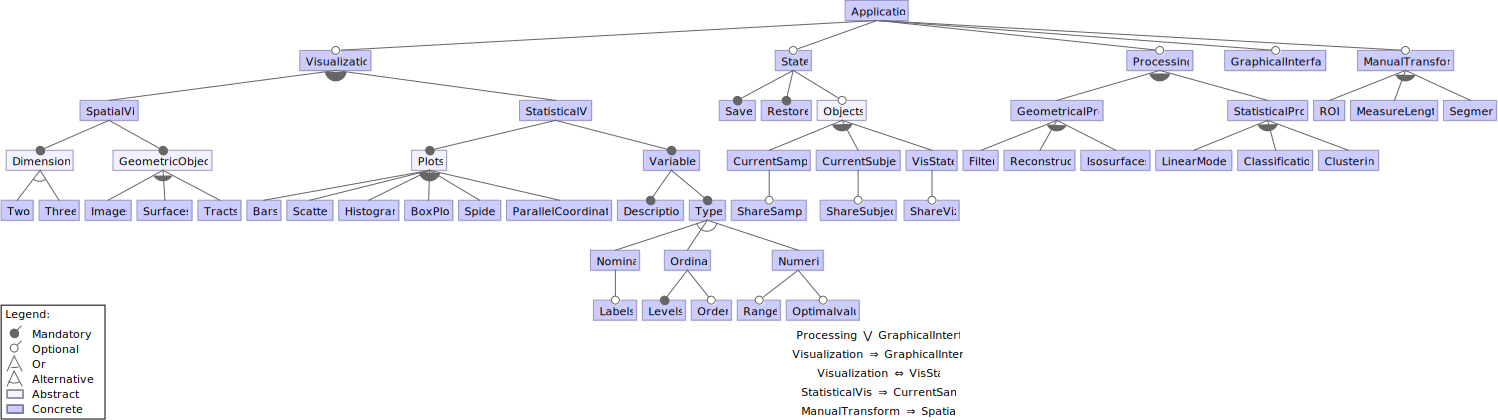
\includegraphics[width=\textwidth]{featureProblem}
\caption{\label{fig_feature_problem}Feature map of the problem space. It illustrates the different features that make up applications for the domain.}
\end{figure}

The main elements in the diagram are

\begin{itemize}
\item Application: The root of the tree, each of the applications in the family are configured based on this tree
\item Interactive Visualization: Most applications will have interactive visualizations as its main component. The exception are applications that prepare data for exploratory analysis. Visualizations can exist for spatial data (usually referred to as scientific visualizations ) or non spatial data (usually referred to as information visualization).
\begin{itemize}
\item Spatial Visualization: These visualizations show spatial objects, this is, objects with coordinates associated to some physical space. Notice this visualizations can be in a plane, with only two coordinates, or a in a full 3d space. These visualizations can display one or several of the listed Geometric Objects.
\item Non Spatial Visualizations: These visualizations represent abstract values in a coordinate system that is not necessarily associated with any physical space. Typical plots found in statistical tools belong here, the diagram shows only some examples. Notice that several of them can be displayed at the same time in order to convey additional aspects of the data. This is specially useful if different views are coordinated. The information displayed in the plots comes from variables. 
\end{itemize}
\item Workflow: Features in this branch can make the exploratory analysis workflow more efficient. 
\begin{itemize}
\item Save Restore: One of the key requirements is being able to split an analysis sessions between several times. Therefore applications should have an state that can be saved and restored. The state can have a reference to the current subject, current sample and the internal state of visualizations. 
\item Log: Applications may write important actions performed by the user to a log. This log can be further improved with textual comments and highlights written by the user. It can afterwards be used to retrieve the process at a later time or to share with colleagues.
\item Communication: Different applications can communicate with each other in order to provide coordinated views from different points. In this way applications can share a subject of interest, a sample of interest, variables of interest or the configuration of spatial visualizations.
\end{itemize}
\item Interface: Most applications are expected to have a graphical interface so that users can interact with it visually. Remember these interfaces should be simple and expose only the functionality required for a specific task. However some applications can be used to process data in batch form, in order to prepare it for future analysis. In this case a command line interface may be enough. 
\item Processing: One of the key steps in the visual analytics loop is data transformation. These transformations can be fully automatic and therefore calculated without the need for user intervention; others will require the intervention of experts.
\begin{itemize}
\item Automatic: These functions may come operate on spatial data, and therefore come from the computational geometry domain, or they may operate on tabular data using techniques from statistics or machine learning. Some examples of these operations are shown in the tree.
\item  Manual Assist: Some operations can't yet be performed reliably in a fully automatic way. In these cases it is necessary to get the expert involved in the systematic transformation of the data. Tools should be designed to make the manual intervention as small as possible, and everything that could be automated should be in order to ease the workload or the expert. An example could be providing an initial estimation automatically and then let the expert make adjustments. Some examples of these operations are presented in the tree: ROI (Region of Interest) definition, length measurement, and manual segmentation.

\end{itemize}

\end{itemize}

Under the feature model some additional restrictions are found. First, applications should either have a graphical interface or perform automatic processing of data. Visualizations require a graphical user interface. Also if visualizations are present they should have an explicit visualization state, at the same time the visualization state must be associated with visualizations. Statistical visualizations require a explicit sample. Finally manual transformations require an spatial visualization. 

These feature model represents a family of applications that can be adapted for several tasks, data types and users. By choosing different features several kinds of applications can be built. Specifically there are applications focused on transforming the data and others focused on visualizing it. Both of these fit at different places of the visual analytics workflow (figure \ref{fig_workflows}). Notice that the model permits applications focused on spatial data, applications focused on tabular data, but also applications that integrate both of them. The sharing nodes in the tree are there to allow users and teams to use several applications to complete more complex analyzes. However coordinating operations is more easily accomplished by having a central coordinator. This central coordinator can also help with the recovery of a previous session by keeping a log of the usage of different applications. In the following section we will show how this platform and the family of applications can be implemented.

% Commonalities and differences in these applications

% Domain Terms

% Use cases

% Feature model


%- Define domain
%-- Examples
%-- Main Features
%-- Relationship to other domains
%- Analysis of existing Applications
%-- Commonalities and Differences
%-- From other domains, need to be compatible
%- Analysis of literatures and experts
%- Domain Terms
%- Domain Concepts
%- Variability of domain concepts
%-- feature model in problem space
% trade offs
% analyzis of combinations

\section{Solution Proposal}

The domain described above requires applications tailored for specific tasks and data, but also requires the integration of data, users and workflows. In order to achieve this, we propose a family of applications and a common platform that integrates them. Because target users have to do exploratory research through several small sessions spread trough a long time, it is critical that the system helps them get up to speed where they left off. Additionally it is crucial to document findings, so that they can be corroborated and socialized. These requires associated finding with the data that supports them, and how they are made evident through the right visualizations. The path to such a finding or insight may involve going trough several applications, and we need to take them all into account. These applications also need to be coordinated in order to make moving from one to the other pleasant, avoiding the need to repeat tasks and therefore allowing the expert to concentrate more easily. We propose a central node which coordinates communication between applications and at the same time keeps a log of the activity of all of them. This log can be improved with annotations from the user, and reviewed at any time. Specific elements from the log can be shared to colleagues and associated to findings. The diagram in figure \ref{fig_deployment} shows the deployment of the proposed system.

\begin{figure}
\centering
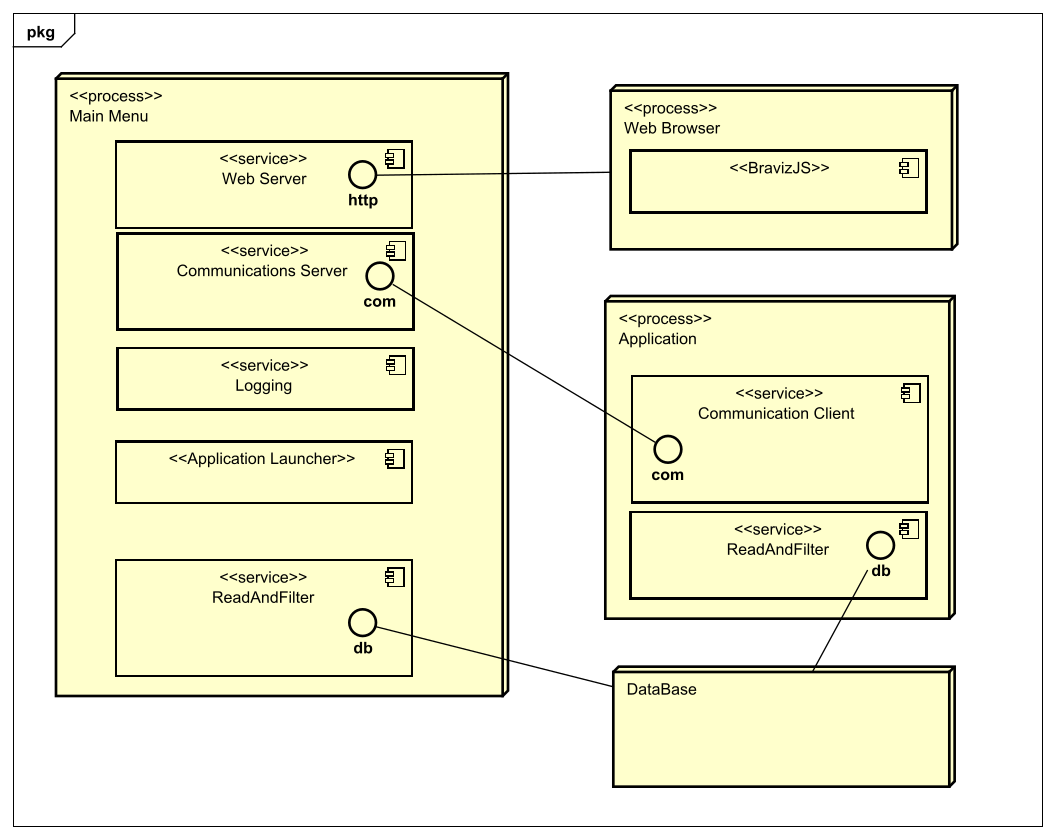
\includegraphics[width=0.9\textwidth]{braviz/BravizDeploy}
\caption{\label{fig_deployment} Deployment diagram of the proposed solution. At the left is the main process, which includes the communication server and logger, to the right there are web-based applications that run on a web server as well as desktop applications each one running on its own process. Notices that all of them share the same databse.}
\end{figure}

The \emph{Main Menu} process behaves as the master of the session. There are two flavors of applications: stand-alone or web based, more details on this later. Finally there is a single database containing the data, this data is visible by all applications, and any transformed data is sent to this same database. This shared database is the first mechanism for coordination between applications, but more fluid integration can be achieved by sharing state across the system. For this purpose all applications connect to the \emph{Main Menu}. This central application also keeps track of important changes done on the other applications and saves them in a log. This log will allow future retrieval and reconstruction of the analysis session. Individual applications and the central node share significant functionality, therefore we expect them to share important parts of code, as for example the module that connects to the database.
 
It can be seen that individual applications support the \emph{explore} use case, while the platform plays the main role in \emph{share} and \emph{review}. In the next chapter we will describe an implementation of the proposed system and later on we will see how it gets used in real projects.

\subsection{Platform}

Exploratory analysis requires iterating trough the data several times, using different tools and looking from different points of view. This is best accomplished by using different applications, but having them all working in the same direction. We propose a set of coordinated applications for this task. Usually changing from one application to another requires has a large overhead. For this reason users try to avoid switching applications, and when it has to be done, they are forced to change their focus to the details of the operation and momentarily forget about the data. We propose an environment when users can move seamless between applications. Even better, multiple applications can be opened at the same time, and what goes on in one will be reflected on the other. If large display real estate is available, there could be multiple points of view active at the same time, and the specialist would just have to move the eyes to see the current data from a different point of view. Even though work happens on several different applications, when reviewing it, it should look as a coherent work-flow. 

During the Visual Analytics cycle shown in figure \ref{fig_workflows} data is constantly transformed and fed back into the process. In the proposed analysis environment there is a single pool of data. All applications read from data from here, expose it to the user, and in case the user requests a transformation the transformed data is fed back into the system. In this way the pool of data is constantly growing and getting richer. Notice that data created by some application can be accessed from any other. This provides a practical mechanism to move data between applications. All applications can share the code that accesses this pool of data, and therefore the user won't have to care about making data compatible with other applications. It can be seen like all applications contribute to this repository of data and at the same way all of them benefit from it, this is the fist way in which the system moves forward as a whole.

Data in this domain is either associated to a subject or to a sample (see figure \ref{fig_datum_class}). During an analysis session users will look at several of them. Ideally each application should provide a different point of view on the same entity. Some of them will provide higher detail, and some will provide lower detail. Some will show mainly spatial data while others will focus on complementary data. The mechanism trough which this is achieved is that when an application changes the current sample or subject, it reports the change to the rest of the running applications. These applications can listen to the message and react to it. Applications may also choose to ignore certain messages at certain times. As always, the user is the most important actor of the system. The system should adapt to the user, and the user should always be in control, and feel like that. If applications over-react to signals they may confuse the user, who may not understand what is going on. Then it is important to make explicit the messaging mechanism, and let the user turn it on, off or fine tune it at will. If done correctly, this mechanism can improve user experience by providing the user the information he is interested in at the right time.

If the above mechanisms are implemented right the set of applications should move forward as a pack. Therefore it would be nice to monitor it as an unique system instead of separate applications. For this reason we can take advantage of the already central position of the message server. Applications may not only send reports when switching focus, but also send messages reporting changes in their internal states just for logging purposes. The purpose of the log is to let users review the workflow and specially the path that led to a discovery. For this reason it is important to display this log to the user in a way that allows him to recall the situation at a glance. The log should also allow annotations such that it can be shared among users. Finally, the crucial pieces of evidence that support a discovery should be identifiable from the log, associated to the discovery and finally attached to a report on such discovery.



%Proposal for Braviz platform
%
%- Data Flow
%- Task
%- Use Case (igual que arriba?)
%- Deployment


\subsection{Applications Family}

Individual applications are where most of the job will be accomplished. We expect to have a very diverse set of applications that adapts to several users and tasks. While each application will be different, there will be all based on common asset. The objective is to create these applications using the techniques from Software Product Line Engineering \autocite{pohl_software_2005}. The feature diagram from figure \ref{fig_feature_problem} show the expected variability from the user perspective. From it we derive a second feature plot (see figure \ref{fig_feature_solution}) that shows the variability of applications from a more technical point of view.  

\begin{figure}
\centering
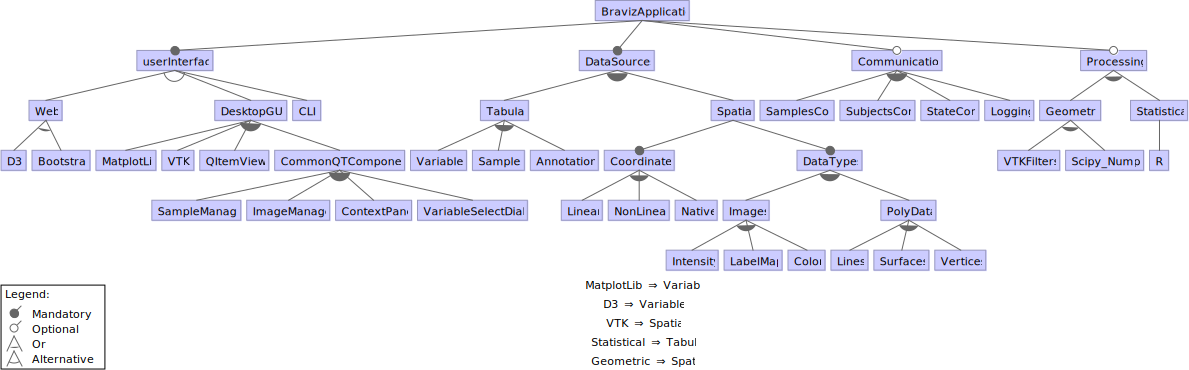
\includegraphics[width=\textwidth]{featureSolution}
\caption{\label{fig_feature_solution}Feature Diagram of the solution space. It shows the available choices of features to create applications in the domain. Choices must be made depending on the task and the user.}
\end{figure}

Notice that this diagram evidences some selections of the technology that will be used in the implementation. VTK \autocite{schroeder_vtk_1998} is the most common scientific visualization framework, and most of the tools we analyzed use it. Given that one of our objectives is to play nice with existing software this comes as a natural choice. In the statistical side, R \autocite{team_r:_2012} is one of the most used statistical software, and it has the advantage of being open source. Because of this it we can connect it to our application, and most importantly, we can ask our users to install it without this imposing a financial burden. We will be using python as the main developing environment, again, because it has become on of the most popular languages in the neuro-science  community. For this reason several packages can we found to perform data processing and reading. An important example is the nipy \autocite{gorgolewski_nipype:_2011-1} suite. There are also robust scientific libraries \autocite{van_der_walt_numpy_2011, jones_scipy:_2001,mckinney_data_2010} available inside this platform as well as libraries for statistical plotting, specifically Matplotlib \autocite{hunter_matplotlib:_2007} and seaborn \autocite{michael_waskom_seaborn:_2015}.

Most of the applications will require a graphical user interface. We propose two alternatives in this case, a web-based user interface or a desktop application. Web interfaces can provide high quality interactive graphics using java-script libraries as D3 \autocite{bostock_d3_2011}, it is also possible to show 3d graphics on web browsers using \emph{webgl} and related libraries as \emph{three.js}, however these technologies are still very young and experimental. On the other side, showing interactive 3D graphics interactively in a desktop client is a mature technology. Additional user interface elements can be created using the QT framework on desktop and the bootstrap framework on web. The decision between web and desktop must be taken depending on the kind of visualization that the application will contain. If complex interactive 3d graphics are required, then the interface must be a desktop one. If non-spatial visualizations are required, it must be analyzed if the specific kind of plot can be better created with D3 or with Matplotlib. In the case of desktop applications, several common components are available. At the current stage these are

\begin{itemize}
\item SampleManager: Handles creation, loading, saving and optionally communication of samples.
\item ImageManager: Allows the user to select an image from the collection of images available in the current project.
\item ContextPanel: A panel that displays values of selected variables for the current subject.
\item VariableSelectDialog: A generic dialog that lets the user search and select variables, as well as review and modify the associated meta-data.
\end{itemize}
If a graphical user interface is not required, a command line based interface should be included. 

Each application may require different data sources. The possible sources are classified in two groups. On one side the application may require access to variables, samples or annotations. 
Variables represent properties of the subjects or samples, and therefore they should have a description to help with its interpretation. There are three main types of variables.
\begin{itemize}
\item Nominal Variables: These variables represent categories of data. They don't necessarily have an order and in general it is not possible to perform arithmetic operations on them. Examples of these are: Gender, City of birth and eye's color.
\item Ordinal Variables: These variables have an associated order but in general it is not possible to perform arithmetic on them. Examples of these are a likert scale (strongly agree, agree, neither agree or disagree, disagree or strongly disagree), months in a year, streets in a city, poker hands or a names in a phone-book.
\item Numerical variables: These variables can me mapped to a subset of the real numbers. They can be further divided into \emph{interval} and  \emph{ratio}. In interval ratio the distance between two values is meaningful, for example temperature in degrees Celsius, dates or coordinates in the globe. These variables can be added and subtracted, and statistics like the arithmetic mean and variance are meaningful. Ratio variables additionally have a meaningful zero or origin. Examples of these are age, speed, height, weight or electric field. It makes sense to multiply two of these values together and therefore statistics like the geometric mean are meaningful.
\end{itemize}

Samples are grouping of subjects which can be used to test an hypothesis only for a specific group, or to compare several groups. Annotations are free-text complementary information of each subject. They can be used to store and keep present information that can't be encoded into variables.

On the other side applications may require access to spatial data. These can be Images or PolyData structures, and they may be required in one or more coordinate systems. There are three possible kinds of images: intensity, where each voxel contain a real number indicating the intensity of a signal or effect; label map, where each voxel contains an integer representing membership to a set; and color images, where each voxel contains a color. Polydata may contain vertices, lines or surfaces. Additionally there may be scalar values associated to each vertex, line, or polygon. 

Spatial data my be shown on a single coordinate system, or the user may have the option to select the best one for the current task. Usually there is a trade-off. Native coordinate systems display data as was acquired, and therefore provide the highest fidelity. Linear registration requires resampling, which add some noise to the data; however it is easier to make comparisons on registered data. Finally non-linear registration provides the highest correspondence between data from different subjects, but adds a significant amount of distortion. This space may be adequate when one wants to compare scalar values at a given location on different subjects, however most of the differences in shape or size will disappear.

Applications may optionally implement communication mechanisms, but are very encouraged to do so as in this way they become more fit to collaborate with other applications in the family, and by doing so enable more complex tasks to be completed by users. Communication may include sending and receiving samples, subjects, complete state or logging messages. The latest are interpreted by the logging module in the central node. Finally applications may include facilities to transform and process data. Statistical processing can be done using R, while geometrical processing can be accomplished using either VTK or the python scientific libraries Numpy and Scipy. 

It may be tempting to create applications that include all possible features, however most likely this will result on overly complex applications which are hard to use by users. Remember applications should first of all be designed to target a concrete task. Features should only be added when they help the task be accomplished. Features should not be added just because they can be added. Simplicity plays a key role. The best applications will be targeted to a single task, and will only include those features that contribute to such task. 

Notice that while there is significant room for variability across applications, it is expected that they all share a large amount of code. By doing this critical pieces of code only need to be implemented and tested once, and then used across the different applications. The result is that application developers only need to worry about the target user and task; while technical details are handled by the reusable components. This separation of concerns will allow us to provide several applications designed for specific analysis tasks and users, on top of a solid foundation. More details about the implementation of the system will be given on chapter \ref{chap_braviz}.


%Proposal for Braviz application family
%
%- Feature model
%-- problem space
%-- solution space
%
%- rationale for each choice
%- when to select each feature
%- how to choose between alternatives